\section{Parallel K-Means}
\label{sec:parallel kmeans}

This section will present results relevant to the GPU parallel K-Means.
Its purpose is to understand how dataset complexity (number of patterns, features and centroids) affect the speed-up of the GPU version over the CPU.
All tests were executed on machine Charlie and the block size was maintained constant at 512.

\subsection{Maximum potential speed-up}

Previously, it was mentioned that the methodology followed for speeding up an application was to first profile the code and identify the portions of code that can be optimized and what fraction of the total computational time they take.
Table \ref{tab:kmeans max speedup} presents statistical results on the theoretical maximum speed-up for the two K-Means phases.
The sequential version of K-Means was executed over a wide spectrum of datasets varying the number of patterns, dimensions and centroids. % cardinality, dimensionality and number of clusters.
The theoretical maximum speed-up is considered to be the overall speed-up of the algorithm if one of its phases had infinite speed-up, i.e. when its time is negligible relative to the other phases.
Analyzing these results it is clear that the labeling phase holds the most potential for optimizations.
Furthermore, the theoretical speed-up also increases with the problem complexity (number of patterns, dimensions and centroids), since, the execution time for the labeling phase with more complex datasets is higher compared to the update phase.
The theoretical speed-up of the update phase is almost negligible when compared to the labeling phase.
This illustrates the importance of profiling the code before proceeding with optimizations, since effort invested in the update phase would yield little effect.

\begin{table}[h]
\centering
\caption{Maximum theoretical speed-up for the labeling and update phases of K-Means based on experimental data. The datasets used range from $1000$ to $500 \: 000$ patterns, from $2$ to $1000$ dimensions and from $2$ to $2048$ centroids.}

\begin{tabular}{lrr}
\toprule
{} &  Labeling phase &  Update phase \\
\midrule
mean  &               540.830750 &                    1.046810 \\
std   &               879.914267 &                    0.083625 \\
min   &                 2.998327 &                    1.000199 \\
25\% percentile &      18.657822 &                    1.001470 \\
50\% percentile &      99.868132 &                    1.010139 \\
75\% percentile &     681.250941 &                    1.056709 \\
max   &              5026.972226 &                    1.519945 \\
\bottomrule
\end{tabular}

\label{tab:kmeans max speedup}
\end{table}


\subsection{Analysis of speed-up}

Observing Figures \ref{fig:kmeans dim 2} and \ref{fig:kmeans dim 200}, it is clear that the number of patterns, dimensions and centroids influence the speed-up.
It should be noted that whenever the number of centroids was superior to $70\%$ of the number of patterns, that particular test case was not executed.
For the simple case of 2 dimensions (Fig \ref{fig:kmeans dim 2}), the speed-up increases with the number of patterns.
However, there is no speed-up when the overall complexity of the datasets is low.
For 2 clusters, there is no speed-up before of $100 \: 000$ patterns.
And even after that mark, the speed-up is not significant.
On the other hand, for a large number of clusters, there is speed-up for any number of patterns processed.
Not only that, that speed-up is highest of any other case with inferior number of clusters.
The reason for this is that the total amount of work increases linearly with the number of clusters but is diluted by the number of threads that can execute simultaneously.

\begin{figure}[hbtp]
    \centering
    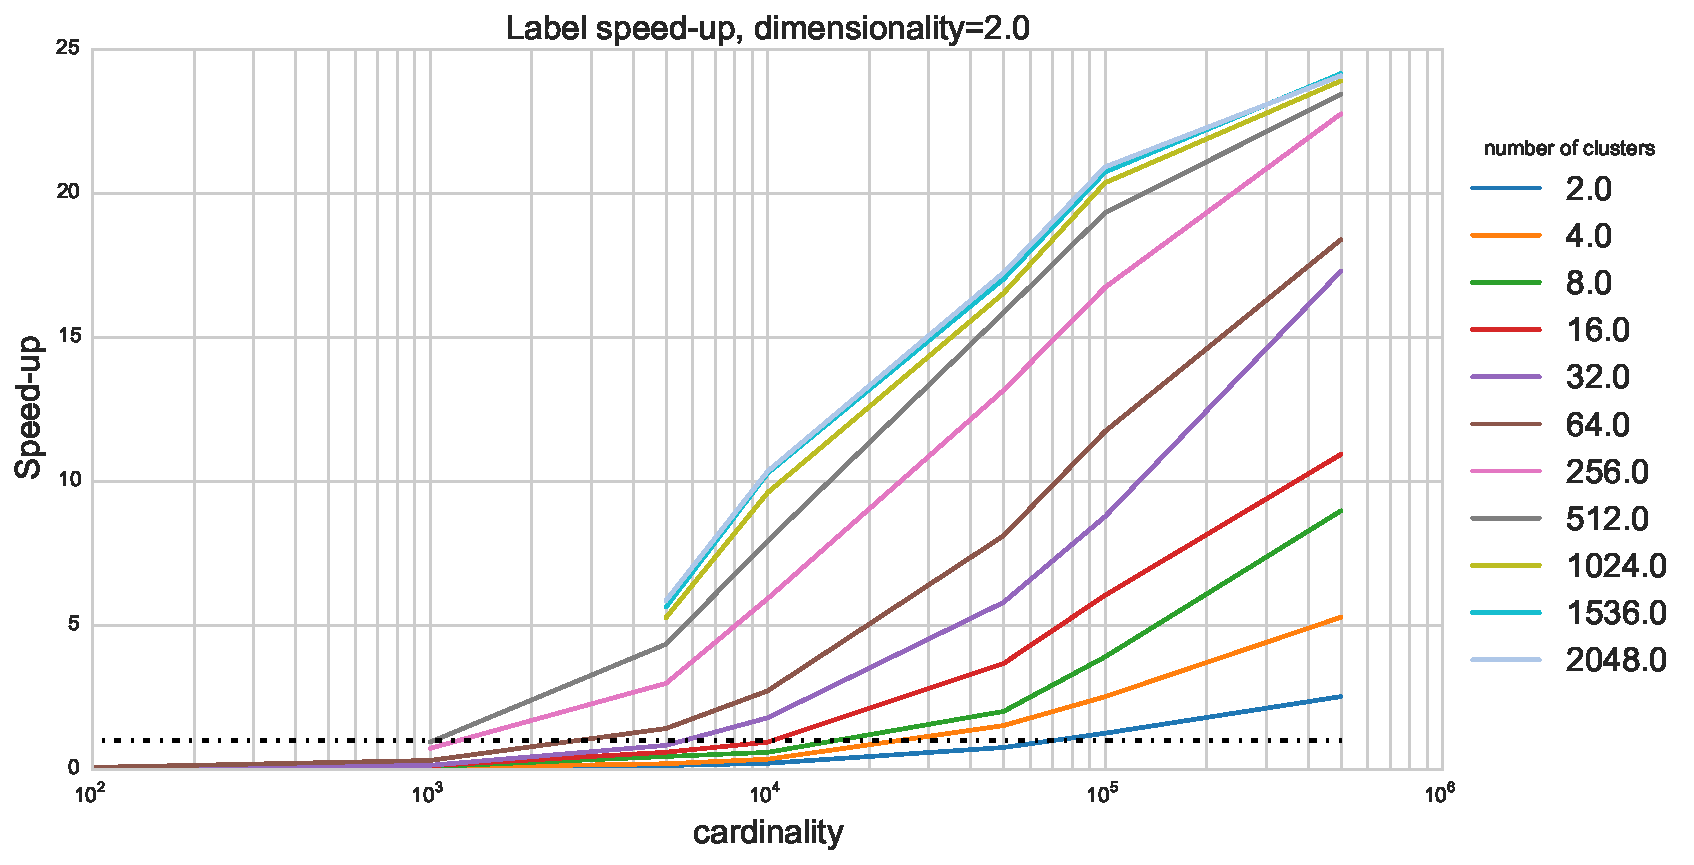
\includegraphics[width=\textwidth]{{{results/kmeans/fixed_dimensions/2.0}}}
    \caption{Speed-up of the labeling phase for datasets of 2 dimensions and varying cardinality and number of clusters. The dotted black line represents a speed-up of one.}
    \label{fig:kmeans dim 2}
\end{figure}

However, as the number of dimensions increases (observe Fig. \ref{fig:kmeans dim 200}), the speed-up increases until a certain number of patterns and then decreases.
Here, the initial number of patterns for which there is a speed-up is lower than in the low dimensionality case and the number of clusters plays less an influence on the speed-up.
It is believed that the reason for this is related to the implementation itself.
The current parallel implementation does not use shared memory, which is fast.
As such, for every computation, each thread fetches the relevant data from global memory which is significantly slower.
As the number of dimensions increases, the amount of data that each thread must fetch also increases.
Furthermore, since the number of dimensions affects both data points and centroids, if the number of dimensions increases by 2 the number of fetches to memory increases by 4.
So, the speed-up increases with the dataset complexity until a point where the number of fetches to memory starts having a very significant effect on the execution time, decreasing the speed-up close to $50\%$.

% As it stands, this implementation of K-Means excels in low-dimensional datasets with a high number of centroids.
% Good performance on a high number of centroids is a desireble thing given the overall context 

\begin{figure}[hbtp]
    \centering
    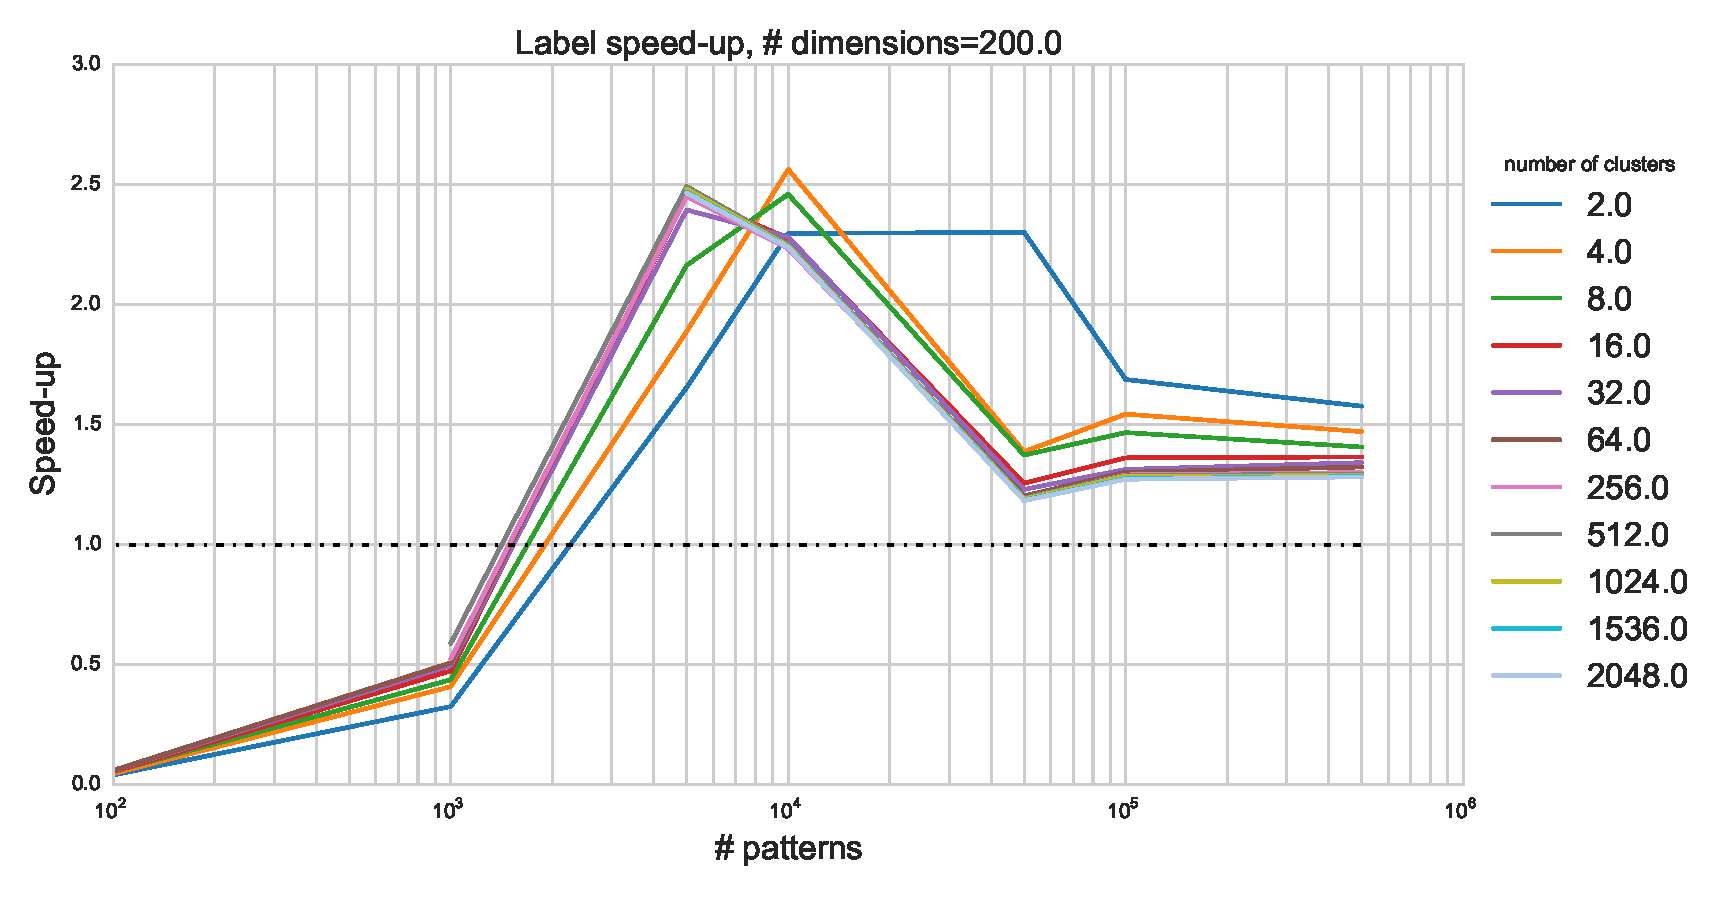
\includegraphics[width=\textwidth]{{{results/kmeans/fixed_dimensions/200.0}}}
    \caption{Speed-up of the labeling phase for datasets of 200 dimensions and varying cardinality and number of clusters. The dotted black line represents a speed-up of one.}
    \label{fig:kmeans dim 200}
\end{figure}

\subsection{Effective bandwidth and computational throughput}
% check devblogs.nvidia.com/parallelforall/how-implement-performance-metrics-cuda-cc/

Effective bandwidth and throughput are two useful metrics to measure the efficiency of CUDA programs.
The effective bandwidth was computed by summing the times of transferring data to and fro the device divided by the total amount of data transfered and is usually represented in GBytes/s.
The computational throughput is usually represented in GFLOP/s (Giga-FLoating-point OPerations per second).
These metrics were computed from the results and a statistical overview is presented in Table \ref{tab:kmeans performance metrics}.
The results refer only to the labeling phase to make a fair comparison between CPU and GPU, although considering both phases would not alter significantly the results since the update phase represents a small fraction of the computational complexity.
The computational throughput of the GPU is more than 3 times higher than that of the CPU, on average.
However, it is interesting to note that the minimum GPU throughput is significantly lower than the CPU.
This is because of what was seen in previous sections, where the dataset complexity is too low for the overhead associated with using the GPU to outweigh the benefit of the parallel computation.
Furthermore, it should be noted that the effective metrics of the GPU are well below the maximum theoretical presented in the device specifications, which are a bandwidth of 288 GB/s and a throughput of 4.29 TFLOP/s.
This suggests that the GPU is underused on the presented test cases. % usage on the presented test cases is still underused.

\begin{table}[ht]
\centering
\caption{Effective bandwidth and computational throughput of labeling phase computed from results taken from running K-Means over datasets whose complexity ranged from $100$ to $10 \: 000 \: 000$ patterns, from $2$ to $1000$ dimensions and from $2$ to $2048$ centroids.}

\begin{tabular}{lrrr}
\toprule
{} &  GPU bandwidth [GB/s] &  GPU throughput [GFLOP/s] &  CPU throughput [GFLOP/s] \\
\midrule
mean             &         2.902388 &    3.655521 &        1.048632 \\
std              &         2.278465 &    4.510252 &        0.330869 \\
min              &         0.001433 &    0.003631 &        0.029959 \\
25\% percentile &         0.567006 &    1.547014 &        0.872651 \\
50\% percentile  &         2.892260 &    1.711037 &        1.179825 \\
75\% percentile  &         5.319831 &    4.168283 &        1.296973 \\
max             &         6.044631 &   21.915104 &        1.447981 \\
\bottomrule
\end{tabular}

\label{tab:kmeans performance metrics}
\end{table}

\subsection{Influence of the number of points per thread}

The number of patterns each thread processes (PPT) may influence performance as well.
To evaluate this hypothesis, several runs over the datasets of $500 \: 000$ patterns with different points per thread were executed.
A brief statistical analysis of the results is presented in Table \ref{tab:kmeans cuda ppt}.
The average speed-up almost doubled when executing 2 PPT.
For more than 2 PPT, the speed-up seemed to decrease with an increase of the number of PPT.
Since the labeling kernel was not optimized for reducing the number of memory calls when processing more than one PTT, the increase in speed-up may be justified by the reduced overhead of calling less blocks of threads.
The fraction of the threads that did not execute any patterns increased with the PPT, which may be the cause for the decrease of speed-up with an increase of PPT after 2.

\begin{table}[h]
\centering
\caption{Speed-up obtained in the labeling phase for different number of patterns per thread (PPT).}


\begin{tabular}{lrrrrr}
\toprule
{} &       {} 	   &   {} 		   &  \textbf{Speed-up}  & {} 		& {}\\
{} &       PPT = 1 &       PPT = 2 &       PPT = 4 &       PPT = 8 &      PPT = 16 \\
\midrule
mean  &   5.898964 &  10.147513 &   3.736146 &   3.113199 &   2.090518 \\
std   &   7.470687 &  13.379909 &   4.027777 &   3.007031 &   1.264650 \\
min   &   1.235194 &   2.457333 &   1.521486 &   1.376941 &   1.258223 \\
25\% percentile  &   1.300021 &   2.561924 &   1.584261 &   1.473213 &   1.363452 \\
50\% percentile  &   2.048436 &   2.704003 &   1.721874 &   1.572580 &   1.432653 \\
75\% percentile  &   4.828922 &   9.321841 &   2.063122 &   1.897468 &   1.696736 \\
max   &  24.151800 &  46.752640 &  12.845526 &   9.943271 &   4.952390 \\
\bottomrule
\end{tabular}

\label{tab:kmeans cuda ppt}
\end{table}